\subsection{Experiment Interfaces}

\subsubsection{Mechanical Interfaces}
\label{sec:4.2.1}
The experiment mounting platform will be attached to the upper rails of the gondola.

% Discuss mounting safety


\begin{figure}[H]
    \centering
	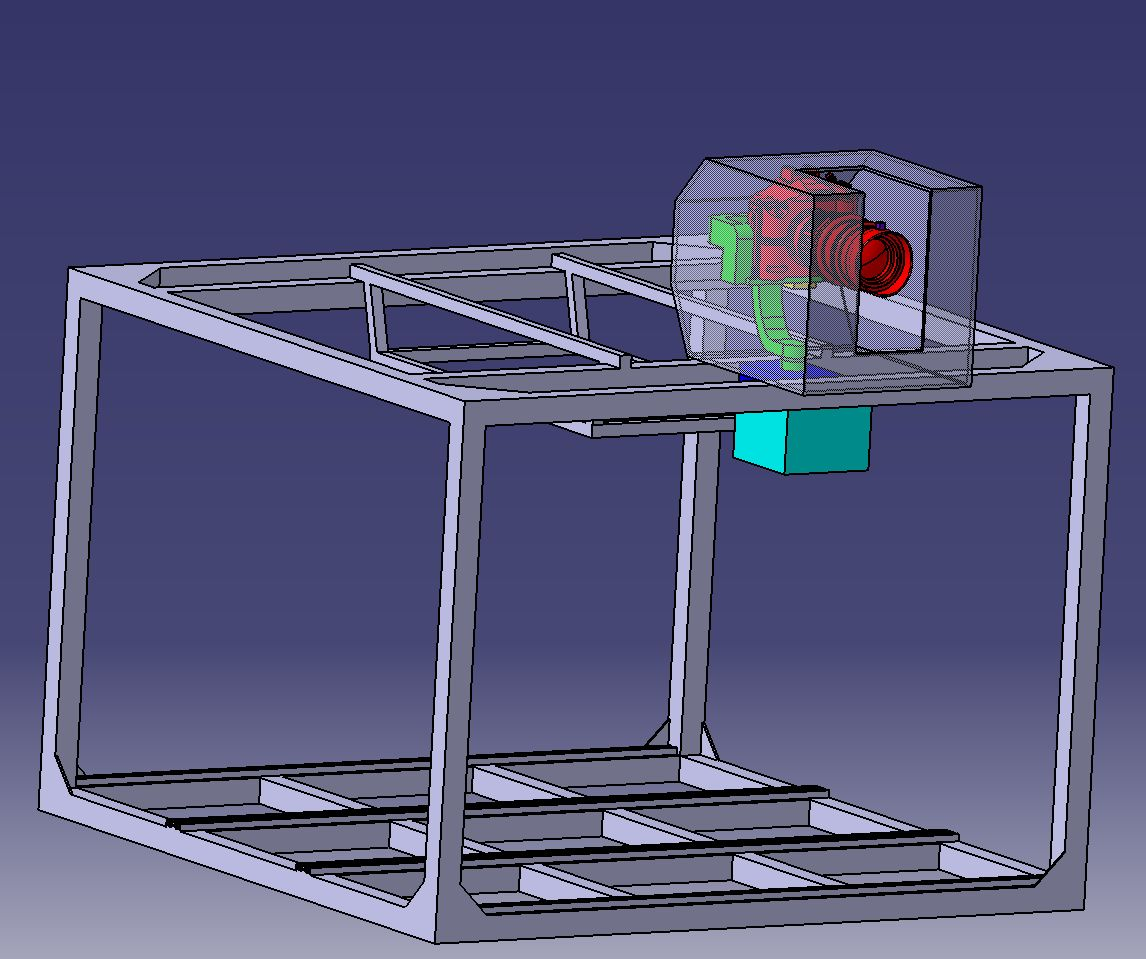
\includegraphics[scale=.8]{4-experiment-design/img/interfaces/Screenshot_Experiment.jpg}
	\caption{Instrument position on gondola}
\end{figure}

\begin{figure}[H]
    \centering
	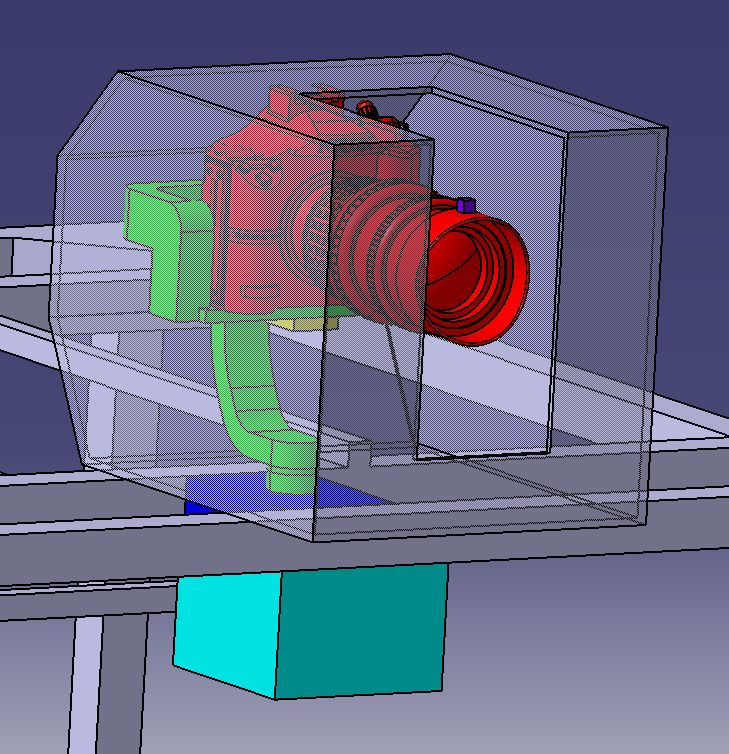
\includegraphics[scale=.8]{4-experiment-design/img/interfaces/Screenshot_Close_Up.jpg}
	\caption{Close up of the instrument mounting}
\end{figure}


% \bigskip
% \input{4-experiment-design/tables/attaching_comp.tex}


\subsubsection{Thermal Interfaces}
\label{sec:4.2.2}


\subsubsection{Electrical Interfaces}
\label{sec:4.2.3}
\textbf{E-link:}\\
The uplink will be used to send occasional commands to control the experiment. One command will be [\hl{TBD}] in size. The TCP/IP protocol will be used for uplink, so the total size of one transmission will be the data plus the TCP header (maximum 480 bits), the IP header (maximum 480 bits) and the Ethernet frame (144 bits). 

$$ bits\, per\, uplink\, packet &\leq [TBD] + 480 + 480 + 144 $$

The downlink will be used to send science and housekeeping data to the ground station. The data in the downlink packet is estimated to be [\hl{TBD}]. For downlink, UPD protocol will be used, as the reliability of the data is not as crucial as during the uplink and to compensate for the size of the data packet. The total size of one packet will be the data plus the UDP header (32 bits), the IP header (maximum 480 bits) and the Ethernet frame (144 bits).

$$ bits\, per\, downlink\, packet &\leq [TBD] + 32 + 480 + 144 $$

\textbf{Power:}
Info about power cables, their length/resistivity and thus power loss, their connection to gondola power relay. 



\textbf{Connectors:}\\

\textbf{Protection:}\\

\textbf{Grounding:}\\


\subsubsection{Radio Frequencies (Optional)}


\subsubsection{Thermal (Optional)}



\raggedbottom